\documentclass[12pt]{article}
%\documentclass[12pt,landscape]{article}


%packages
%\usepackage{latexsym}
\usepackage{graphicx}
\usepackage{color}
\usepackage{amsmath}
\usepackage{dsfont}
\usepackage{placeins}
\usepackage{amssymb}
\usepackage{wasysym}
\usepackage{abstract}
\usepackage{hyperref}
\usepackage{etoolbox}
\usepackage{datetime}
\usepackage{xcolor}
\usepackage{alphalph}
\usepackage{centernot}
\settimeformat{ampmtime}

%\usepackage{pstricks,pst-node,pst-tree}

%\usepackage{algpseudocode}
%\usepackage{amsthm}
%\usepackage{hyperref}
%\usepackage{mathrsfs}
%\usepackage{amsfonts}
%\usepackage{bbding}
%\usepackage{listings}
%\usepackage{appendix}
\usepackage[margin=1in]{geometry}
%\geometry{papersize={8.5in,11in},total={6.5in,9in}}
%\usepackage{cancel}
%\usepackage{algorithmic, algorithm}

\makeatletter
\def\maxwidth{ %
  \ifdim\Gin@nat@width>\linewidth
    \linewidth
  \else
    \Gin@nat@width
  \fi
}
\makeatother

\definecolor{fgcolor}{rgb}{0.345, 0.345, 0.345}
\newcommand{\hlnum}[1]{\textcolor[rgb]{0.686,0.059,0.569}{#1}}%
\newcommand{\hlstr}[1]{\textcolor[rgb]{0.192,0.494,0.8}{#1}}%
\newcommand{\hlcom}[1]{\textcolor[rgb]{0.678,0.584,0.686}{\textit{#1}}}%
\newcommand{\hlopt}[1]{\textcolor[rgb]{0,0,0}{#1}}%
\newcommand{\hlstd}[1]{\textcolor[rgb]{0.345,0.345,0.345}{#1}}%
\newcommand{\hlkwa}[1]{\textcolor[rgb]{0.161,0.373,0.58}{\textbf{#1}}}%
\newcommand{\hlkwb}[1]{\textcolor[rgb]{0.69,0.353,0.396}{#1}}%
\newcommand{\hlkwc}[1]{\textcolor[rgb]{0.333,0.667,0.333}{#1}}%
\newcommand{\hlkwd}[1]{\textcolor[rgb]{0.737,0.353,0.396}{\textbf{#1}}}%

\usepackage{framed}
\makeatletter
\newenvironment{kframe}{%
 \def\at@end@of@kframe{}%
 \ifinner\ifhmode%
  \def\at@end@of@kframe{\end{minipage}}%
  \begin{minipage}{\columnwidth}%
 \fi\fi%
 \def\FrameCommand##1{\hskip\@totalleftmargin \hskip-\fboxsep
 \colorbox{shadecolor}{##1}\hskip-\fboxsep
     % There is no \\@totalrightmargin, so:
     \hskip-\linewidth \hskip-\@totalleftmargin \hskip\columnwidth}%
 \MakeFramed {\advance\hsize-\width
   \@totalleftmargin\z@ \linewidth\hsize
   \@setminipage}}%
 {\par\unskip\endMakeFramed%
 \at@end@of@kframe}
\makeatother

\definecolor{shadecolor}{rgb}{.77, .77, .77}
\definecolor{messagecolor}{rgb}{0, 0, 0}
\definecolor{warningcolor}{rgb}{1, 0, 1}
\definecolor{errorcolor}{rgb}{1, 0, 0}
\newenvironment{knitrout}{}{} % an empty environment to be redefined in TeX

\usepackage{alltt}
\usepackage[T1]{fontenc}

\newcommand{\qu}[1]{``#1''}
\newcounter{probnum}
\setcounter{probnum}{1}

%create definition to allow local margin changes
\def\changemargin#1#2{\list{}{\rightmargin#2\leftmargin#1}\item[]}
\let\endchangemargin=\endlist 

%allow equations to span multiple pages
\allowdisplaybreaks

%define colors and color typesetting conveniences
\definecolor{gray}{rgb}{0.5,0.5,0.5}
\definecolor{black}{rgb}{0,0,0}
\definecolor{white}{rgb}{1,1,1}
\definecolor{blue}{rgb}{0.5,0.5,1}
\newcommand{\inblue}[1]{\color{blue}#1 \color{black}}
\definecolor{green}{rgb}{0.133,0.545,0.133}
\newcommand{\ingreen}[1]{\color{green}#1 \color{black}}
\definecolor{yellow}{rgb}{1,1,0}
\newcommand{\inyellow}[1]{\color{yellow}#1 \color{black}}
\definecolor{orange}{rgb}{0.9,0.649,0}
\newcommand{\inorange}[1]{\color{orange}#1 \color{black}}
\definecolor{red}{rgb}{1,0.133,0.133}
\newcommand{\inred}[1]{\color{red}#1 \color{black}}
\definecolor{purple}{rgb}{0.58,0,0.827}
\newcommand{\inpurple}[1]{\color{purple}#1 \color{black}}
\definecolor{backgcode}{rgb}{0.97,0.97,0.8}
\definecolor{Brown}{cmyk}{0,0.81,1,0.60}
\definecolor{OliveGreen}{cmyk}{0.64,0,0.95,0.40}
\definecolor{CadetBlue}{cmyk}{0.62,0.57,0.23,0}

%define new math operators
\DeclareMathOperator*{\argmax}{arg\,max~}
\DeclareMathOperator*{\argmin}{arg\,min~}
\DeclareMathOperator*{\argsup}{arg\,sup~}
\DeclareMathOperator*{\arginf}{arg\,inf~}
\DeclareMathOperator*{\convolution}{\text{\Huge{$\ast$}}}
\newcommand{\infconv}[2]{\convolution^\infty_{#1 = 1} #2}
%true functions

%%%% GENERAL SHORTCUTS

%shortcuts for pure typesetting conveniences
\newcommand{\bv}[1]{\boldsymbol{#1}}

%shortcuts for compound constants
\newcommand{\BetaDistrConst}{\dfrac{\Gamma(\alpha + \beta)}{\Gamma(\alpha)\Gamma(\beta)}}
\newcommand{\NormDistrConst}{\dfrac{1}{\sqrt{2\pi\sigma^2}}}

%shortcuts for conventional symbols
\newcommand{\tsq}{\tau^2}
\newcommand{\tsqh}{\hat{\tau}^2}
\newcommand{\sigsq}{\sigma^2}
\newcommand{\sigsqsq}{\parens{\sigma^2}^2}
\newcommand{\sigsqovern}{\dfrac{\sigsq}{n}}
\newcommand{\tausq}{\tau^2}
\newcommand{\tausqalpha}{\tau^2_\alpha}
\newcommand{\tausqbeta}{\tau^2_\beta}
\newcommand{\tausqsigma}{\tau^2_\sigma}
\newcommand{\betasq}{\beta^2}
\newcommand{\sigsqvec}{\bv{\sigma}^2}
\newcommand{\sigsqhat}{\hat{\sigma}^2}
\newcommand{\sigsqhatmlebayes}{\sigsqhat_{\text{Bayes, MLE}}}
\newcommand{\sigsqhatmle}[1]{\sigsqhat_{#1, \text{MLE}}}
\newcommand{\bSigma}{\bv{\Sigma}}
\newcommand{\bSigmainv}{\bSigma^{-1}}
\newcommand{\thetavec}{\bv{\theta}}
\newcommand{\thetahat}{\hat{\theta}}
\newcommand{\thetahatmle}{\hat{\theta}_{\mathrm{MLE}}}
\newcommand{\thetavechatmle}{\hat{\thetavec}_{\mathrm{MLE}}}
\newcommand{\muhat}{\hat{\mu}}
\newcommand{\musq}{\mu^2}
\newcommand{\muvec}{\bv{\mu}}
\newcommand{\muhatmle}{\muhat_{\text{MLE}}}
\newcommand{\lambdahat}{\hat{\lambda}}
\newcommand{\lambdahatmle}{\lambdahat_{\text{MLE}}}
\newcommand{\etavec}{\bv{\eta}}
\newcommand{\alphavec}{\bv{\alpha}}
\newcommand{\minimaxdec}{\delta^*_{\mathrm{mm}}}
\newcommand{\ybar}{\bar{y}}
\newcommand{\xbar}{\bar{x}}
\newcommand{\Xbar}{\bar{X}}
\newcommand{\phat}{\hat{p}}
\newcommand{\Phat}{\hat{P}}
\newcommand{\Zbar}{\bar{Z}}
\newcommand{\iid}{~{\buildrel iid \over \sim}~}
\newcommand{\inddist}{~{\buildrel ind \over \sim}~}
\newcommand{\approxdist}{~{\buildrel approx \over \sim}~}
\newcommand{\equalsindist}{~{\buildrel d \over =}~}
\newcommand{\loglik}[1]{\ell\parens{#1}}
\newcommand{\thetahatkminone}{\thetahat^{(k-1)}}
\newcommand{\thetahatkplusone}{\thetahat^{(k+1)}}
\newcommand{\thetahatk}{\thetahat^{(k)}}
\newcommand{\half}{\frac{1}{2}}
\newcommand{\third}{\frac{1}{3}}
\newcommand{\twothirds}{\frac{2}{3}}
\newcommand{\fourth}{\frac{1}{4}}
\newcommand{\fifth}{\frac{1}{5}}
\newcommand{\sixth}{\frac{1}{6}}

%shortcuts for vector and matrix notation
\newcommand{\A}{\bv{A}}
\newcommand{\At}{\A^T}
\newcommand{\Ainv}{\inverse{\A}}
\newcommand{\B}{\bv{B}}
\newcommand{\K}{\bv{K}}
\newcommand{\Kt}{\K^T}
\newcommand{\Kinv}{\inverse{K}}
\newcommand{\Kinvt}{(\Kinv)^T}
\newcommand{\M}{\bv{M}}
\newcommand{\Bt}{\B^T}
\newcommand{\Q}{\bv{Q}}
\renewcommand{\H}{\bv{H}}
\newcommand{\Qt}{\Q^T}
\newcommand{\R}{\bv{R}}
\newcommand{\Rt}{\R^T}
\newcommand{\Z}{\bv{Z}}
\newcommand{\X}{\bv{X}}
\newcommand{\U}{\bv{U}}
\newcommand{\V}{\bv{V}}
\newcommand{\Xsub}{\X_{\text{(sub)}}}
\newcommand{\Xsubadj}{\X_{\text{(sub,adj)}}}
\newcommand{\I}{\bv{I}}
\newcommand{\Y}{\bv{Y}}
\newcommand{\sigsqI}{\sigsq\I}
\renewcommand{\P}{\bv{P}}
\newcommand{\Psub}{\P_{\text{(sub)}}}
\newcommand{\Pt}{\P^T}
\newcommand{\Pii}{P_{ii}}
\newcommand{\Pij}{P_{ij}}
\newcommand{\IminP}{(\I-\P)}
\newcommand{\Xt}{\bv{X}^T}
\newcommand{\XtX}{\Xt\X}
\newcommand{\XtXinv}{\parens{\Xt\X}^{-1}}
\newcommand{\XtXinvXt}{\XtXinv\Xt}
\newcommand{\XXtXinvXt}{\X\XtXinvXt}
\newcommand{\x}{\bv{x}}
\newcommand{\w}{\bv{w}}
\renewcommand{\b}{\bv{b}}
\newcommand{\onevec}{\bv{1}}
\newcommand{\zerovec}{\bv{0}}
\newcommand{\oneton}{1, \ldots, n}
\newcommand{\yoneton}{y_1, \ldots, y_n}
\newcommand{\yonetonorder}{y_{(1)}, \ldots, y_{(n)}}
\newcommand{\Yoneton}{Y_1, \ldots, Y_n}
\newcommand{\iinoneton}{i \in \braces{\oneton}}
\newcommand{\onetom}{1, \ldots, m}
\newcommand{\jinonetom}{j \in \braces{\onetom}}
\newcommand{\xoneton}{x_1, \ldots, x_n}
\newcommand{\Xoneton}{X_1, \ldots, X_n}
\newcommand{\xt}{\x^T}
\newcommand{\y}{\bv{y}}
\newcommand{\yt}{\y^T}
\renewcommand{\c}{\bv{c}}
\newcommand{\ct}{\c^T}
\newcommand{\tstar}{\bv{t}^*}
\renewcommand{\u}{\bv{u}}
\renewcommand{\v}{\bv{v}}
\renewcommand{\a}{\bv{a}}
\newcommand{\s}{\bv{s}}
\newcommand{\yadj}{\y_{\text{(adj)}}}
\newcommand{\xjadj}{\x_{j\text{(adj)}}}
\newcommand{\xjadjM}{\x_{j \perp M}}
\newcommand{\yhat}{\hat{\y}}
\newcommand{\yhatsub}{\yhat_{\text{(sub)}}}
\newcommand{\yhatstar}{\yhat^*}
\newcommand{\yhatstarnew}{\yhatstar_{\text{new}}}
\newcommand{\z}{\bv{z}}
\newcommand{\zt}{\z^T}
\newcommand{\bb}{\bv{b}}
\newcommand{\bbt}{\bb^T}
\newcommand{\bbeta}{\bv{\beta}}
\newcommand{\beps}{\bv{\epsilon}}
\newcommand{\bepst}{\beps^T}
\newcommand{\e}{\bv{e}}
\newcommand{\Mofy}{\M(\y)}
\newcommand{\KofAlpha}{K(\alpha)}
\newcommand{\ellset}{\mathcal{L}}
\newcommand{\oneminalph}{1-\alpha}
\newcommand{\SSE}{\text{SSE}}
\newcommand{\SSEsub}{\text{SSE}_{\text{(sub)}}}
\newcommand{\MSE}{\text{MSE}}
\newcommand{\RMSE}{\text{RMSE}}
\newcommand{\SSR}{\text{SSR}}
\newcommand{\SST}{\text{SST}}
\newcommand{\JSest}{\delta_{\text{JS}}(\x)}
\newcommand{\Bayesest}{\delta_{\text{Bayes}}(\x)}
\newcommand{\EmpBayesest}{\delta_{\text{EmpBayes}}(\x)}
\newcommand{\BLUPest}{\delta_{\text{BLUP}}}
\newcommand{\MLEest}[1]{\hat{#1}_{\text{MLE}}}

%shortcuts for Linear Algebra stuff (i.e. vectors and matrices)
\newcommand{\twovec}[2]{\bracks{\begin{array}{c} #1 \\ #2 \end{array}}}
\newcommand{\threevec}[3]{\bracks{\begin{array}{c} #1 \\ #2 \\ #3 \end{array}}}
\newcommand{\fivevec}[5]{\bracks{\begin{array}{c} #1 \\ #2 \\ #3 \\ #4 \\ #5 \end{array}}}
\newcommand{\twobytwomat}[4]{\bracks{\begin{array}{cc} #1 & #2 \\ #3 & #4 \end{array}}}
\newcommand{\threebytwomat}[6]{\bracks{\begin{array}{cc} #1 & #2 \\ #3 & #4 \\ #5 & #6 \end{array}}}

%shortcuts for conventional compound symbols
\newcommand{\thetainthetas}{\theta \in \Theta}
\newcommand{\reals}{\mathbb{R}}
\newcommand{\complexes}{\mathbb{C}}
\newcommand{\rationals}{\mathbb{Q}}
\newcommand{\integers}{\mathbb{Z}}
\newcommand{\naturals}{\mathbb{N}}
\newcommand{\forallninN}{~~\forall n \in \naturals}
\newcommand{\forallxinN}[1]{~~\forall #1 \in \reals}
\newcommand{\matrixdims}[2]{\in \reals^{\,#1 \times #2}}
\newcommand{\inRn}[1]{\in \reals^{\,#1}}
\newcommand{\mathimplies}{\quad\Rightarrow\quad}
\newcommand{\mathlogicequiv}{\quad\Leftrightarrow\quad}
\newcommand{\eqncomment}[1]{\quad \text{(#1)}}
\newcommand{\limitn}{\lim_{n \rightarrow \infty}}
\newcommand{\limitN}{\lim_{N \rightarrow \infty}}
\newcommand{\limitd}{\lim_{d \rightarrow \infty}}
\newcommand{\limitt}{\lim_{t \rightarrow \infty}}
\newcommand{\limitsupn}{\limsup_{n \rightarrow \infty}~}
\newcommand{\limitinfn}{\liminf_{n \rightarrow \infty}~}
\newcommand{\limitk}{\lim_{k \rightarrow \infty}}
\newcommand{\limsupn}{\limsup_{n \rightarrow \infty}}
\newcommand{\limsupk}{\limsup_{k \rightarrow \infty}}
\newcommand{\floor}[1]{\left\lfloor #1 \right\rfloor}
\newcommand{\ceil}[1]{\left\lceil #1 \right\rceil}

%shortcuts for environments
\newcommand{\beqn}{\vspace{-0.25cm}\begin{eqnarray*}}
\newcommand{\eeqn}{\end{eqnarray*}}
\newcommand{\bneqn}{\vspace{-0.25cm}\begin{eqnarray}}
\newcommand{\eneqn}{\end{eqnarray}}

%shortcuts for mini environments
\newcommand{\parens}[1]{\left(#1\right)}
\newcommand{\squared}[1]{\parens{#1}^2}
\newcommand{\tothepow}[2]{\parens{#1}^{#2}}
\newcommand{\prob}[1]{\mathbb{P}\parens{#1}}
\newcommand{\cprob}[2]{\prob{#1~|~#2}}
\newcommand{\littleo}[1]{o\parens{#1}}
\newcommand{\bigo}[1]{O\parens{#1}}
\newcommand{\Lp}[1]{\mathbb{L}^{#1}}
\renewcommand{\arcsin}[1]{\text{arcsin}\parens{#1}}
\newcommand{\prodonen}[2]{\bracks{\prod_{#1=1}^n #2}}
\newcommand{\mysum}[4]{\sum_{#1=#2}^{#3} #4}
\newcommand{\sumonen}[2]{\sum_{#1=1}^n #2}
\newcommand{\infsum}[2]{\sum_{#1=1}^\infty #2}
\newcommand{\infprod}[2]{\prod_{#1=1}^\infty #2}
\newcommand{\infunion}[2]{\bigcup_{#1=1}^\infty #2}
\newcommand{\infinter}[2]{\bigcap_{#1=1}^\infty #2}
\newcommand{\infintegral}[2]{\int^\infty_{-\infty} #2 ~\text{d}#1}
\newcommand{\supthetas}[1]{\sup_{\thetainthetas}\braces{#1}}
\newcommand{\bracks}[1]{\left[#1\right]}
\newcommand{\braces}[1]{\left\{#1\right\}}
\newcommand{\set}[1]{\left\{#1\right\}}
\newcommand{\abss}[1]{\left|#1\right|}
\newcommand{\norm}[1]{\left|\left|#1\right|\right|}
\newcommand{\normsq}[1]{\norm{#1}^2}
\newcommand{\inverse}[1]{\parens{#1}^{-1}}
\newcommand{\rowof}[2]{\parens{#1}_{#2\cdot}}

%shortcuts for functionals
\newcommand{\realcomp}[1]{\text{Re}\bracks{#1}}
\newcommand{\imagcomp}[1]{\text{Im}\bracks{#1}}
\newcommand{\range}[1]{\text{range}\bracks{#1}}
\newcommand{\colsp}[1]{\text{colsp}\bracks{#1}}
\newcommand{\rowsp}[1]{\text{rowsp}\bracks{#1}}
\newcommand{\tr}[1]{\text{tr}\bracks{#1}}
\newcommand{\rank}[1]{\text{rank}\bracks{#1}}
\newcommand{\proj}[2]{\text{Proj}_{#1}\bracks{#2}}
\newcommand{\projcolspX}[1]{\text{Proj}_{\colsp{\X}}\bracks{#1}}
\newcommand{\median}[1]{\text{median}\bracks{#1}}
\newcommand{\mean}[1]{\text{mean}\bracks{#1}}
\newcommand{\dime}[1]{\text{dim}\bracks{#1}}
\renewcommand{\det}[1]{\text{det}\bracks{#1}}
\newcommand{\expe}[1]{\mathbb{E}\bracks{#1}}
\newcommand{\expeabs}[1]{\expe{\abss{#1}}}
\newcommand{\expesub}[2]{\mathbb{E}_{#1}\bracks{#2}}
\newcommand{\indic}[1]{\mathds{1}_{#1}}
\newcommand{\var}[1]{\mathbb{V}\text{ar}\bracks{#1}}
\newcommand{\cov}[2]{\mathbb{C}\text{ov}\bracks{#1, #2}}
\newcommand{\corr}[2]{\text{Corr}\bracks{#1, #2}}
\newcommand{\se}[1]{\mathbb{S}\text{E}\bracks{#1}}
\newcommand{\seest}[1]{\hat{\mathbb{S}\text{E}}\bracks{#1}}
\newcommand{\bias}[1]{\text{Bias}\bracks{#1}}
\newcommand{\derivop}[2]{\dfrac{\text{d}}{\text{d} #1}\bracks{#2}}
\newcommand{\partialop}[2]{\dfrac{\partial}{\partial #1}\bracks{#2}}
\newcommand{\secpartialop}[2]{\dfrac{\partial^2}{\partial #1^2}\bracks{#2}}
\newcommand{\mixpartialop}[3]{\dfrac{\partial^2}{\partial #1 \partial #2}\bracks{#3}}

%shortcuts for functions
\renewcommand{\exp}[1]{\mathrm{exp}\parens{#1}}
\renewcommand{\cos}[1]{\text{cos}\parens{#1}}
\renewcommand{\sin}[1]{\text{sin}\parens{#1}}
\newcommand{\sign}[1]{\text{sign}\parens{#1}}
\newcommand{\are}[1]{\mathrm{ARE}\parens{#1}}
\newcommand{\natlog}[1]{\ln\parens{#1}}
\newcommand{\oneover}[1]{\frac{1}{#1}}
\newcommand{\overtwo}[1]{\frac{#1}{2}}
\newcommand{\overn}[1]{\frac{#1}{n}}
\newcommand{\oneoversqrt}[1]{\oneover{\sqrt{#1}}}
\newcommand{\sqd}[1]{\parens{#1}^2}
\newcommand{\loss}[1]{\ell\parens{\theta, #1}}
\newcommand{\losstwo}[2]{\ell\parens{#1, #2}}
\newcommand{\cf}{\phi(t)}

%English language specific shortcuts
\newcommand{\ie}{\textit{i.e.} }
\newcommand{\AKA}{\textit{AKA} }
\renewcommand{\iff}{\textit{iff}}
\newcommand{\eg}{\textit{e.g.} }
\newcommand{\st}{\textit{s.t.} }
\newcommand{\wrt}{\textit{w.r.t.} }
\newcommand{\mathst}{~~\text{\st}~~}
\newcommand{\mathand}{~~\text{and}~~}
\newcommand{\ala}{\textit{a la} }
\newcommand{\ppp}{posterior predictive p-value}
\newcommand{\dd}{dataset-to-dataset}

%shortcuts for distribution titles
\newcommand{\logistic}[2]{\mathrm{Logistic}\parens{#1,\,#2}}
\newcommand{\bernoulli}[1]{\mathrm{Bernoulli}\parens{#1}}
\newcommand{\betanot}[2]{\mathrm{Beta}\parens{#1,\,#2}}
\newcommand{\stdbetanot}{\betanot{\alpha}{\beta}}
\newcommand{\multnormnot}[3]{\mathcal{N}_{#1}\parens{#2,\,#3}}
\newcommand{\normnot}[2]{\mathcal{N}\parens{#1,\,#2}}
\newcommand{\classicnormnot}{\normnot{\mu}{\sigsq}}
\newcommand{\stdnormnot}{\normnot{0}{1}}
\newcommand{\uniformdiscrete}[1]{\mathrm{Uniform}\parens{\braces{#1}}}
\newcommand{\uniform}[2]{\mathrm{U}\parens{#1,\,#2}}
\newcommand{\stduniform}{\uniform{0}{1}}
\newcommand{\geometric}[1]{\mathrm{Geometric}\parens{#1}}
\newcommand{\hypergeometric}[3]{\mathrm{Hypergeometric}\parens{#1,\,#2,\,#3}}
\newcommand{\exponential}[1]{\mathrm{Exp}\parens{#1}}
\newcommand{\gammadist}[2]{\mathrm{Gamma}\parens{#1, #2}}
\newcommand{\poisson}[1]{\mathrm{Poisson}\parens{#1}}
\newcommand{\binomial}[2]{\mathrm{Binomial}\parens{#1,\,#2}}
\newcommand{\negbin}[2]{\mathrm{NegBin}\parens{#1,\,#2}}
\newcommand{\rayleigh}[1]{\mathrm{Rayleigh}\parens{#1}}
\newcommand{\multinomial}[2]{\mathrm{Multinomial}\parens{#1,\,#2}}
\newcommand{\gammanot}[2]{\mathrm{Gamma}\parens{#1,\,#2}}
\newcommand{\cauchynot}[2]{\text{Cauchy}\parens{#1,\,#2}}
\newcommand{\invchisqnot}[1]{\text{Inv}\chisq{#1}}
\newcommand{\invscaledchisqnot}[2]{\text{ScaledInv}\ncchisq{#1}{#2}}
\newcommand{\invgammanot}[2]{\text{InvGamma}\parens{#1,\,#2}}
\newcommand{\chisq}[1]{\chi^2_{#1}}
\newcommand{\ncchisq}[2]{\chi^2_{#1}\parens{#2}}
\newcommand{\ncF}[3]{F_{#1,#2}\parens{#3}}

%shortcuts for PDF's of common distributions
\newcommand{\logisticpdf}[3]{\oneover{#3}\dfrac{\exp{-\dfrac{#1 - #2}{#3}}}{\parens{1+\exp{-\dfrac{#1 - #2}{#3}}}^2}}
\newcommand{\betapdf}[3]{\dfrac{\Gamma(#2 + #3)}{\Gamma(#2)\Gamma(#3)}#1^{#2-1} (1-#1)^{#3-1}}
\newcommand{\normpdf}[3]{\frac{1}{\sqrt{2\pi#3}}\exp{-\frac{1}{2#3}(#1 - #2)^2}}
\newcommand{\normpdfvarone}[2]{\dfrac{1}{\sqrt{2\pi}}e^{-\half(#1 - #2)^2}}
\newcommand{\chisqpdf}[2]{\dfrac{1}{2^{#2/2}\Gamma(#2/2)}\; {#1}^{#2/2-1} e^{-#1/2}}
\newcommand{\invchisqpdf}[2]{\dfrac{2^{-\overtwo{#1}}}{\Gamma(#2/2)}\,{#1}^{-\overtwo{#2}-1}  e^{-\oneover{2 #1}}}
\newcommand{\exponentialpdf}[2]{#2\exp{-#2#1}}
\newcommand{\poissonpdf}[2]{\dfrac{e^{-#1} #1^{#2}}{#2!}}
\newcommand{\binomialpdf}[3]{\binom{#2}{#1}#3^{#1}(1-#3)^{#2-#1}}
\newcommand{\rayleighpdf}[2]{\dfrac{#1}{#2^2}\exp{-\dfrac{#1^2}{2 #2^2}}}
\newcommand{\gammapdf}[3]{\dfrac{#3^#2}{\Gamma\parens{#2}}#1^{#2-1}\exp{-#3 #1}}
\newcommand{\cauchypdf}[3]{\oneover{\pi} \dfrac{#3}{\parens{#1-#2}^2 + #3^2}}
\newcommand{\Gammaf}[1]{\Gamma\parens{#1}}

%shortcuts for miscellaneous typesetting conveniences
\newcommand{\notesref}[1]{\marginpar{\color{gray}\tt #1\color{black}}}

%%%% DOMAIN-SPECIFIC SHORTCUTS

%Real analysis related shortcuts
\newcommand{\zeroonecl}{\bracks{0,1}}
\newcommand{\forallepsgrzero}{\forall \epsilon > 0~~}
\newcommand{\lessthaneps}{< \epsilon}
\newcommand{\fraccomp}[1]{\text{frac}\bracks{#1}}

%Bayesian related shortcuts
\newcommand{\yrep}{y^{\text{rep}}}
\newcommand{\yrepisq}{(\yrep_i)^2}
\newcommand{\yrepvec}{\bv{y}^{\text{rep}}}


%Probability shortcuts
\newcommand{\SigField}{\mathcal{F}}
\newcommand{\ProbMap}{\mathcal{P}}
\newcommand{\probtrinity}{\parens{\Omega, \SigField, \ProbMap}}
\newcommand{\convp}{~{\buildrel p \over \rightarrow}~}
\newcommand{\convLp}[1]{~{\buildrel \Lp{#1} \over \rightarrow}~}
\newcommand{\nconvp}{~{\buildrel p \over \nrightarrow}~}
\newcommand{\convae}{~{\buildrel a.e. \over \longrightarrow}~}
\newcommand{\convau}{~{\buildrel a.u. \over \longrightarrow}~}
\newcommand{\nconvau}{~{\buildrel a.u. \over \nrightarrow}~}
\newcommand{\nconvae}{~{\buildrel a.e. \over \nrightarrow}~}
\newcommand{\convd}{~{\buildrel \mathcal{D} \over \rightarrow}~}
\newcommand{\nconvd}{~{\buildrel \mathcal{D} \over \nrightarrow}~}
\newcommand{\withprob}{~~\text{w.p.}~~}
\newcommand{\io}{~~\text{i.o.}}

\newcommand{\Acl}{\bar{A}}
\newcommand{\ENcl}{\bar{E}_N}
\newcommand{\diam}[1]{\text{diam}\parens{#1}}

\newcommand{\taua}{\tau_a}

\newcommand{\myint}[4]{\int_{#2}^{#3} #4 \,\text{d}#1}
\newcommand{\laplacet}[1]{\mathscr{L}\bracks{#1}}
\newcommand{\laplaceinvt}[1]{\mathscr{L}^{-1}\bracks{#1}}
\renewcommand{\min}[1]{\text{min}\braces{#1}}
\renewcommand{\max}[1]{\text{max}\braces{#1}}

\newcommand{\Vbar}[1]{\bar{V}\parens{#1}}
\newcommand{\expnegrtau}{\exp{-r\tau}}

%%% problem typesetting
\definecolor{darkgrey}{rgb}{0.10,0.10,0.9}

\newcommand{\problem}[1]{\noindent \colorbox{black}{{\color{yellow} \large{\textsf{\textbf{Problem \arabic{probnum}}}}~}} \addtocounter{probnum}{1} \vspace{0.2cm} \\ \iftoggle{professormode}{}{\color{darkgrey}} #1}

\newcommand{\easysubproblem}[1]{\ingreen{\item} \iftoggle{professormode}{}{\color{darkgrey}} [easy] #1 \color{black} }
\newcommand{\intermediatesubproblem}[1]{\inorange{\item} \iftoggle{professormode}{}{\color{darkgrey}} [harder] #1 \color{black} }
\newcommand{\hardsubproblem}[1]{\inred{\item} \iftoggle{professormode}{}{\color{darkgrey}} [difficult] #1 \color{black} }
\newcommand{\extracreditsubproblem}[1]{\inpurple{\item} \iftoggle{professormode}{}{\color{darkgrey}} [E.C.] #1 \color{black} }


\newcommand{\spc}[1]{\iftoggle{professormode}{\\ \vspace{#1cm}}{\\ \vspace{-0.3cm}}}

\makeatletter
\newalphalph{\alphmult}[mult]{\@alph}{26}
\renewcommand{\labelenumi}{(\alphmult{\value{enumi}})}

\newcommand{\support}[1]{\text{Supp}\bracks{#1}}
\newcommand{\mode}[1]{\text{Mode}\bracks{#1}}
\newcommand{\IQR}[1]{\text{IQR}\bracks{#1}}
\newcommand{\quantile}[2]{\text{Quantile}\bracks{#1,\,#2}}


\newcommand{\instr}{\small Your answer will consist of a string (e.g. \texttt{aebgd}) where the order of the letters does not matter nor does upper / lowercase. \normalsize}

\title{Math 390.4 / 650.3 Spring 2020 \\ Midterm Examination Two}
\author{Professor Adam Kapelner}

\date{Thursday, May 14, 2020}

\begin{document}
\maketitle

%\noindent Full Name \line(1,0){410}

\thispagestyle{empty}

\section*{Code of Academic Integrity}

\footnotesize
Since the college is an academic community, its fundamental purpose is the pursuit of knowledge. Essential to the success of this educational mission is a commitment to the principles of academic integrity. Every member of the college community is responsible for upholding the highest standards of honesty at all times. Students, as members of the community, are also responsible for adhering to the principles and spirit of the following Code of Academic Integrity.

Activities that have the effect or intention of interfering with education, pursuit of knowledge, or fair evaluation of a student's performance are prohibited. Examples of such activities include but are not limited to the following definitions:

\paragraph{Cheating} Using or attempting to use unauthorized assistance, material, or study aids in examinations or other academic work or preventing, or attempting to prevent, another from using authorized assistance, material, or study aids. Example: using an unauthorized cheat sheet in a quiz or exam, altering a graded exam and resubmitting it for a better grade, etc.
\\

\noindent By taking this exam, you acknowledge and agree to uphold this Code of Academic Integrity. \\

%\begin{center}
%\line(1,0){250} ~~~ \line(1,0){100}\\
%~~~~~~~~~~~~~~~~~~~~~signature~~~~~~~~~~~~~~~~~~~~~~~~~~~~~~~~~~~~~~~~~~~~~ date
%\end{center}

\normalsize

\section*{Instructions}

This exam has 146 total points, is 120 minutes (variable time per question) and closed-book. You are allowed \textbf{two} pages (front and back) of a \qu{cheat sheet}, one table of reference and scrap paper and a graphing calculator. Please read the questions carefully. No food is allowed, only drinks. %If the question reads \qu{compute,} this means the solution will be a number otherwise you can leave the answer in \textit{any} widely accepted mathematical notation which could be resolved to an exact or approximate number with the use of a computer. I advise you to skip problems marked \qu{[Extra Credit]} until you have finished the other questions on the exam, then loop back and plug in all the holes. I also advise you to use pencil. The exam is 100 points total plus extra credit. Partial credit will be granted for incomplete answers on most of the questions. \fbox{Box} in your final answers. Good luck!

\pagebreak




\problem [10min] Consider the following causal diagrams A, B and C below. In each diagram, all three events x, y, z have other causes that are not displayed.


\begin{figure}[htp]
\centering
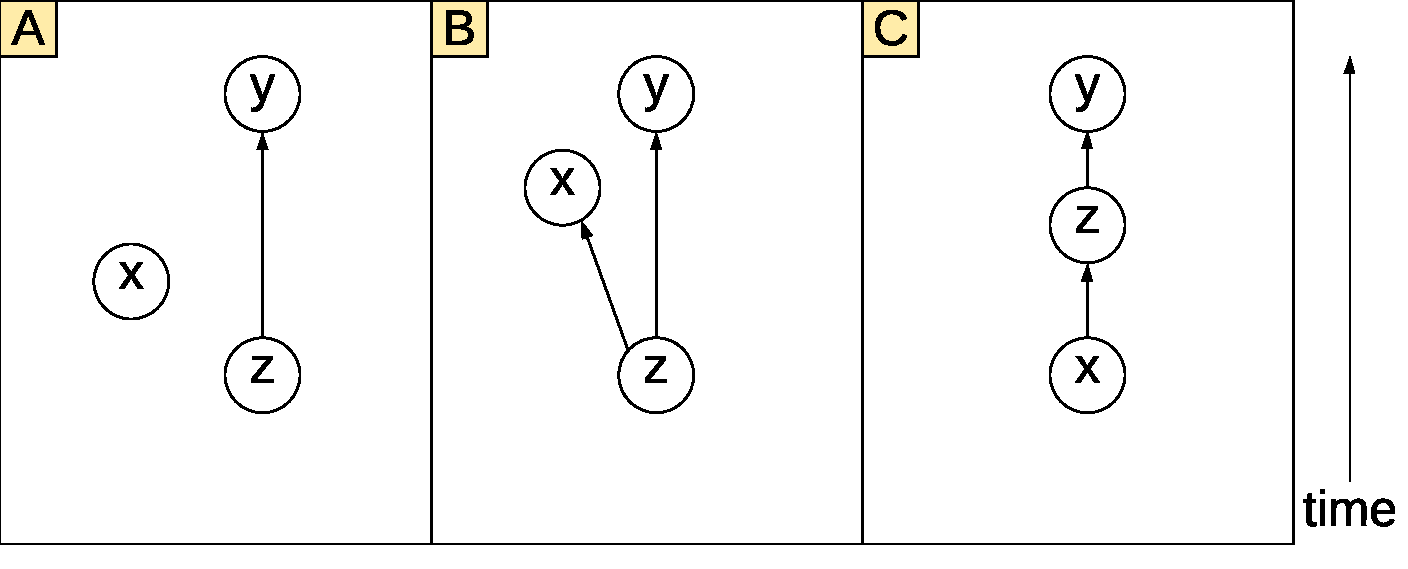
\includegraphics[width=4in]{basic_causal_diagrams}
\end{figure}

\vspace{-.8cm}
\benum

\subquestionwithpoints{13} Record the letter(s) of all the following that are \textbf{true}. 

\begin{enumerate}[(a)]
%\setcounter{enumi}{3}
\item In diagram A, x and y could be spuriously correlated.
\item In diagram A, x and y are correlated.
\item In diagram A, z causes y.
\item In diagram B, x and y could be spuriously correlated.
\item In diagram B, x and y are correlated.
\item In diagram A, x causes y.
\item In diagram C, x and y could be spuriously correlated.
\item In diagram C, x and y are correlated.
\item In diagram C, z could cause x.
\item In diagram A, x causes z and x causes y.
\item Let y be number of car accidents daily in New York City, let z be daily rainfall in New York City and let x be the phase of the moon in degrees. The most likely causal diagram reflecting this situation is A.
\item Let y be number of car accidents daily in New York City, let z be daily rainfall in New York City and let x be the number of people working from home. The most likely causal diagram reflecting this situation is B.
\item Let y be number of car accidents daily in New York City, let z be daily rainfall in New York City and let x be the number of people working from home. The most likely causal diagram reflecting this situation is C.
\end{enumerate}
\eenum\instr\pagebreak

%%%%%%%%%%%%%%%%%%%%%%%%


\problem [11min] Consider the same causal diagrams A, B and C below. In each diagram, all three events x, y, z have other causes that are not displayed.


\begin{figure}[htp]
\centering
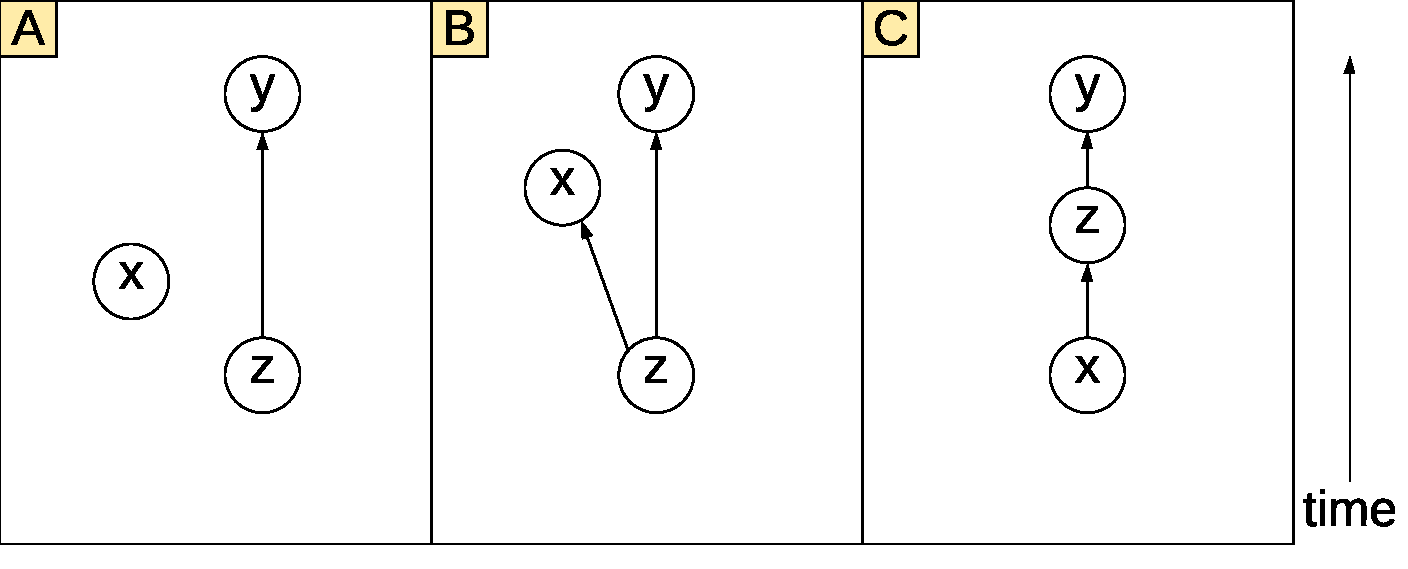
\includegraphics[width=4in]{basic_causal_diagrams}
\end{figure}


Consider the following two predictive models fit by OLS:

\beqn
&[I]& ~~~ \yhat^I = b_0^I + b_1^I x \\
&[II]& ~~~ \yhat^{II} = b_0^{II} + b_1^{II} x + b_2^{II} z
\eeqn


\benum

\subquestionwithpoints{8} Record the letter(s) of all the following that are \textbf{true}. 

\begin{enumerate}[(a)]
%\setcounter{enumi}{3}
\item In causal diagram A, $b_1^I x \approx b_1^{II} x \approx 0$.
\item In causal diagram B, $b_1^I x \approx b_1^{II} x \approx 0$.
\item In causal diagram C, $b_1^I x \approx b_1^{II} x \approx 0$.
\item In causal diagram B, $b_1^I x \neq b_1^{II} x \approx 0$.
\item In causal diagram C, $b_1^I x \neq b_1^{II} x \approx 0$.
\item In all causal diagrams, model [II] performs better out of sample.
\end{enumerate}

The following statements are true about the most correct interpretation of $b_1^I$ for causal diagram B for two observations, O1 and O2.

\begin{enumerate}[(a)]
\setcounter{enumi}{6}
\item O1 and O2 must be sampled in same way as the observations in $\mathbb{D}$ and O2's $x$ measurement is one unit higher than O1's $x$ unit, then the $y$ value of O2 will be on average $b_1^I$ higher than O1 assuming the linear model is true.
\item O1 and O2 must be sampled in same way as the observations in $\mathbb{D}$ and O1 and O2 have the same $x$ and then I manipulate the $x$ value of O2 to be one higher than O1, then the $y$ value of O2 will be on average $b_1^I$ higher than O1 assuming the linear model is true.
\end{enumerate}
\eenum\instr\pagebreak

%%%%%%%%%%%%%%%%%%%%%%%%

\problem [11min] In lab 10 we worked with a data from an accounting firm. The tables were bills, payments and discounts. The bills for one customer and the discounts table is below. The \texttt{discount\_id} column references the \texttt{id} column in the discounts table.

\begin{lstlisting}
> billsA[order(discount_id)]
         id   due_date invoice_date    amount discount_id
1: 16294508 2017-06-25   2017-06-25  99476.43     7302585
2: 17129704 2017-07-29   2017-06-29  99475.01     7564949
3: 15247786 2015-09-18   2015-08-19  99484.62     8218876
4: 17096637 2016-02-02   2016-01-03  99668.94     8806662
5: 17222576 2016-09-15   2016-08-16  99476.93     8806662
6: 16797375 2017-01-29   2016-12-30 116487.16     8806662
> discounts[order(id)]
         id num_days pct_off days_until_discount
 1: 6098612       20      NA                  NA
 2: 6386294      120      NA                  NA
 3: 6609438       NA       1                   7
 4: 7197225       60      NA                  NA
 5: 7302585       NA      NA                  NA
 6: 7708050       NA      NA                  NA
 7: 7833213       10      NA                   5
 8: 8295837       14      NA                  10
 9: 8496508       10       2                  15
10: 8583519        0       2                  NA
11: 8610918        1      NA                  NA
12: 8784190       NA      NA                  30
13: 8806662       30      NA                  NA
14: 8951244       NA      NA                  NA
15: 8988984       60      NA                  NA
\end{lstlisting}
\vspace{-1cm}
\benum


\subquestionwithpoints{12} Each of the following are short for \qu{If we were to do a \line(1,0){50}~of billsA and discounts, we would create a table with \line(1,0){50}}. Record the letter(s) of all the following that are \textbf{true}. 


\begin{enumerate}[(a)]
\item left join / 8 columns.
\item left join / 9 columns.
\item left join / 6 rows.
\item left join / 2 rows.
\item right join / 17 rows.
\item right join / 15 rows.
\item inner join / 2 rows.
\item inner join / 4 rows.
\item inner join / 21 rows.
\item full join / 2 rows.
\item full join / 21 rows.
\item full join / $>$21 rows.
\end{enumerate}
\eenum\instr\pagebreak

%%%%%%%%%%%%%%%%%%%%%%%%

\problem [11min] Here is a dataset about weather:


\begin{figure}[htp]
\centering
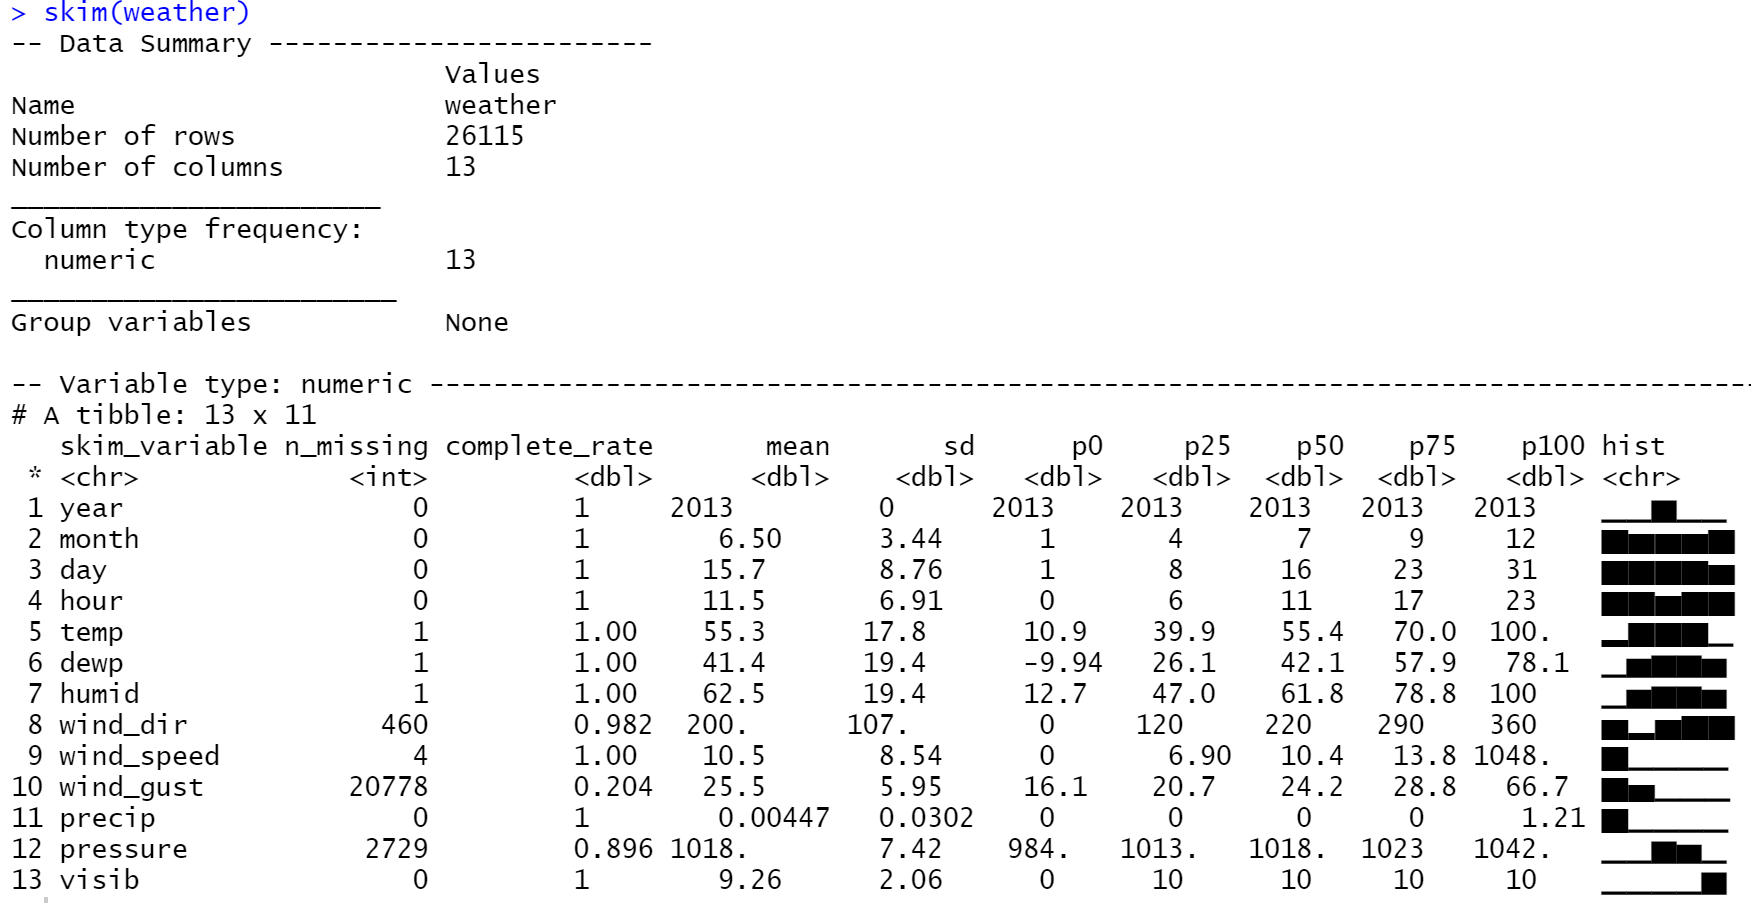
\includegraphics[width=6in]{weather_data.png}
\end{figure}

\benum

\subquestionwithpoints{10} Record the letter(s) of all the following that are \textbf{true}. 


\begin{enumerate}[(a)]
\item If listwise deletion would be used, there would be $n = 5,337$ observations left.
\item If \texttt{wind\_gust} were dropped, there would be less imputations that would have to be made.
\item It would be good practice to drop the observations that have missingness in \texttt{temp}, \texttt{dewp} and \texttt{humid}.
\item If \texttt{wind\_gust} were the response variable, then $n = 5,337$.
\item If \texttt{wind\_gust} were the response variable, and listwise deletion was used, then $n \geq 2141$.
\item If imputation via \texttt{missForest} were used on the \texttt{weather} data frame, the resulting data frame would have $n = 26,115$ observations. \\~\\
If each of these columns contained measurements that were features in a model and we were to both impute and record missingness, the resulting $\X$ matrix in $\mathbb{D}$ would have \line(1,0){20}~columns:
\item 13
\item 16
\item 20
\item 26
\end{enumerate}
\eenum\instr\pagebreak

%%%%%%%%%%%%%%%%%%%%%%%%

\problem [11min] Let $p + 1 = 501$ of features that are all standardized and $n > p + 1$. Let $f(\x) = \x\bbeta$, the first entry of $\x$ is one always, let $\delta$ be a non-trivial amount of homoskedastic noise and $\bbeta = \bracks{\beta_0~\beta_1~\ldots~\beta_{500}}^\top = \bracks{-5~5~4~3~2~1~\zerovec_{495}}^\top$. Consider the usual definition of SSE as the sum of squared error, $\mathcal{H} = \braces{\w^\top \x~:~ \w \in \reals^{p + 1}}$ and all the following algorithms that produce an estimate of $\bbeta$ via:

\beqn
\mathcal{A}_1 &:& \b^{\mathcal{A}_1} = \argmin_{\w \in \reals^{p + 1}}\braces{SSE} \\
\mathcal{A}_2 &:& \b^{\mathcal{A}_2} = \argmin_{\w \in \reals^{p + 1}}\braces{SSE + \sum_{j=1}^{p + 1} |w_j|} \\
\mathcal{A}_3 &:& \b^{\mathcal{A}_3} = \argmin_{\w \in \reals^{p + 1}}\braces{SSE + \sum_{j=1}^{p + 1} w_j^2} \\
\mathcal{A}_4 &:& \b^{\mathcal{A}_4} = \argmin_{\w \in \reals^{p + 1}}\braces{SSE + \half \sum_{j=1}^{p + 1} |w_j| + \half\sum_{j=1}^{p + 1} w_j^2} 
\eeqn

\benum

\subquestionwithpoints{12} Record the letter(s) of all the following that are \textbf{true}. 


\begin{enumerate}[(a)]
\item $\b^{\mathcal{A}_1} = \inverse{\X^\top \X + \I}\X^\top \y$.
\item $\b^{\mathcal{A}_2} = \inverse{\X^\top \X + \I}\X^\top \y$.
\item $\b^{\mathcal{A}_3} = \inverse{\X^\top \X + \I}\X^\top \y$.
\item The OLS algorithm will fail in this setting.
\item $\mathcal{A}_4$ is elastic net regression with $\alpha = \half$.
\item Out of sample, $\mathcal{A}_2, \mathcal{A}_3$ and $\mathcal{A}_4$ will have higher predictive performance than $\mathcal{A}_1$.
\item $\mathcal{A}_2$ likely produces an estimate of $\bbeta$ with more zero entries than $\mathcal{A}_4$.
\item $\mathcal{A}_3$ likely produces an estimate of $\bbeta$ with more zero entries than $\mathcal{A}_4$.
\item $\mathcal{A}_2$ is the most straightforward algorithm that could be used to locate variables that affect the response.
\item $\norm{\bracks{b^{\mathcal{A}_1}_6, b^{\mathcal{A}_1}_7, \ldots, b^{\mathcal{A}_1}_{500}}^\top} < \norm{\bracks{b^{\mathcal{A}_2}_6, b^{\mathcal{A}_2}_7, \ldots, b^{\mathcal{A}_2}_{500}}^\top}$
\item $\norm{\bracks{b^{\mathcal{A}_2}_6, b^{\mathcal{A}_2}_7, \ldots, b^{\mathcal{A}_2}_{500}}^\top} < \norm{\bracks{b^{\mathcal{A}_3}_6, b^{\mathcal{A}_3}_7, \ldots, b^{\mathcal{A}_3}_{500}}^\top}$
\item $\norm{\bracks{b^{\mathcal{A}_4}_6, b^{\mathcal{A}_4}_7, \ldots, b^{\mathcal{A}_4}_{500}}^\top} < \norm{\bracks{b^{\mathcal{A}_1}_6, b^{\mathcal{A}_1}_7, \ldots, b^{\mathcal{A}_1}_{500}}^\top}$
\end{enumerate}
\eenum\instr\pagebreak

%%%%%%%%%%%%%%%%%%%%%%%%

\problem [11min] Assume the response is a real number. In class we studied the following three decompositions of MSE in the modeling context where $\delta$ was realized from a mean-centered r.v. with variance $\sigsq$ independent of the value of $\x$:

\beqn
&[I]& ~~MSE(\x_*) = \sigsq + (f(\x_*) - g(\x_*))^2 \\
&[II]& ~~MSE(\x_*) = \sigsq + \bias{G(\x_*)}^2 + \var{G(\x_*)} \\
&[III]& ~~MSE = \sigsq + \expesub{\mathcal{X}}{\bias{G(\x_*)}^2} + \expesub{\mathcal{X}}{\var{G(\x_*)}} \\
\eeqn

\benum
\subquestionwithpoints{17} Record the letter(s) of all the following that are \textbf{true}. 

\begin{enumerate}[(a)]
\item In I and II, the new observation $\x_*$ was considered drawn from a random universe.
\item In I and II, the training set $\mathbb{D}$ was considered drawn from a random universe.
\item In II and III, the training set $\mathbb{D}$ was considered drawn from a random universe.
\item In II, the responses $\y$ were considered drawn from a random universe.
\item In III, the responses $\y$ were considered drawn from a random universe.
\item In II, the design matrix $\X$ was considered drawn from a random universe.
\item In III, the design matrix $\X$ was considered drawn from a random universe.\\~\\
In general...
\item the $\bias{G(\x_*)}$ term is low for OLS.
\item the $\bias{G(\x_*)}$ term is low for CART.
\item the $\bias{G(\x_*)}$ term is low for a bag of CART models.
\item the $\bias{G(\x_*)}$ term is low for RF.
\item the $\var{G(\x_*)}$ term is low for OLS.
\item the $\var{G(\x_*)}$ term is low for CART.
\item the $\var{G(\x_*)}$ term is low for bag of CART models.
\item the $\var{G(\x_*)}$ term is low for RF.
\item the $\var{G(\x_*)}$ term is lower for CART than it is for a bag of CART models.
\item the $\var{G(\x_*)}$ term is lower for RF than it is for a bag of CART models.
\end{enumerate}
\eenum\instr\pagebreak

%%%%%%%%%%%%%%%%%%%%%%%%

\problem [11min] Consider the following RF model output:

\begin{lstlisting}
YARF v1.0 for classification
Missing data feature ON.
500 trees, training data n = 2000 and p = 99 
Model construction completed within 0.08 minutes.
OOB results on all observations as a confusion matrix:
           predicted 0 predicted 1 model errors
actual 0      1425.000      77.000        0.051
actual 1       192.000     306.000        0.386
use errors       0.119       0.201        0.134

\end{lstlisting}
\vspace{-1cm}
\benum
%    Accuracy: 86.55%

\subquestionwithpoints{20} Record the letter(s) of all the following that are \textbf{true}. 


\begin{enumerate}[(a)]
\item $\mathcal{Y} = \braces{0,1}$.
\item The features that are important in this model are simple to ascertain.
\item The best estimate of this model's accuracy in-sample is less than 86.6\%.
\item The best estimate of this model's accuracy in-sample is more than 86.6\%.
\item The best estimate of this model's accuracy oos is 86.6\%.
\item This RF model will be more accurate oos if it was rebuilt with $M > 500$.
\item This RF model will be less accurate oos if it was rebuilt with $M > 500$.
\item This RF model will be more accurate if $p_{\text{try}} = 99$.
\item When predicting in the future, if there were 100 samples where $y=1$, this model would predict incorrectly 38.6\% of the time.
\item When predicting in the future, if there were 100 samples where $y=1$, this model would predict incorrectly 20.1\% of the time.
\item When predicting in the future, if there were 100 samples where $\hat{y}=1$, this model would predict incorrectly 38.6\% of the time.
\item When predicting in the future, if there were 100 samples where $\hat{y}=1$, this model would predict incorrectly 20.1\% of the time.
\item The oos precision of this model is 79.9\%.
\item The oos recall of this model is 79.9\%.
\item The oos FDR estimate of this model is 11.9\%.
\item The oos FOR estimate of this model is 11.9\%.
\item If the cost of the false positive is greater than the cost of a false negative, this would be a good model to use in the real world.
\item The AUC for this model can be calculated given the output above.
\item The OOB results were calculated on about 2/3 of the total number of observations, $n=2000$.
\item The predictions from each of the $M=500$ constituent trees in this model are positive correlated.
\end{enumerate}
\eenum\instr\pagebreak

%%%%%%%%%%%%%%%%%%%%%%%%

\problem [11min] Let $\mathcal{Y} = \braces{0,1}$ and employ the following algorithm on training data $\mathbb{D}$:

\beqn
\mathcal{A} &:& \b = \argmin_{\w \in \reals^{p + 1}}\braces{\prod_{i=1}^n \tothepow{\oneover{1 + e^{-\w^\top \x_i}}}{y_i} \tothepow{\oneover{1 + e^{\w^\top \x_i}}}{1 - y_i}}
\eeqn

\benum

\subquestionwithpoints{13} Record the letter(s) of all the following that are \textbf{true}. 


\begin{enumerate}[(a)]
\item This algorithm has a closed-form solution for $\b$ as a function of $\X$ and $\y$.
\item $R^2$ is an interpretable metric in this model.
\item This algorithm has hyperparameter(s) that need to be specified before running.
\item This algorithm is called \qu{logistic regression}.
\item The $\b$ that is returned by this algorithm may have numerical error.
\item This algorithm makes statistical assumptions about the training data.
\item The $\b$ returned by this algorithm allows us to compute probability estimates of $\cprob{Y_* = 1}{\x_*} = \b\x_*$.
\item If $\b\x_{*_1} > \b\x_{*_2}$ that implies that the model's estimate for the probability of the response being one for observation $\x_{*_1}$ is higher than for observations $\x_{*_2}$.\\

Consider the following output of $\mathcal{A}$ on the training data $\mathbb{D}$:
 
\begin{lstlisting}
> b
         (Intercept)            x1                   x2
         -10.0175573            0.5971474            0.3090818
\end{lstlisting}

\item If $x_* = \bracks{0~0}$ then the probability estimate of $Y_* = 1$ will be very low.
\item Using the above output, one can compute the Brier score for training data $\mathbb{D}$.
\item Using the above output, one can compute an ROC curve for this model.
\item $g_0(\x) = 0$ for this model.
\item $g_0(\x) = \ybar$ for this model.
\end{enumerate}
\eenum\instr\pagebreak

%%%%%%%%%%%%%%%%%%%%%%%%

\problem [11min] Consider the boston housing data that has response as the median home value and $n = 506$ and $p = 13$. We fit a regression tree model fit setting $N_0 = 200$. Here is the tree visualized:


\begin{figure}[htp]
\centering
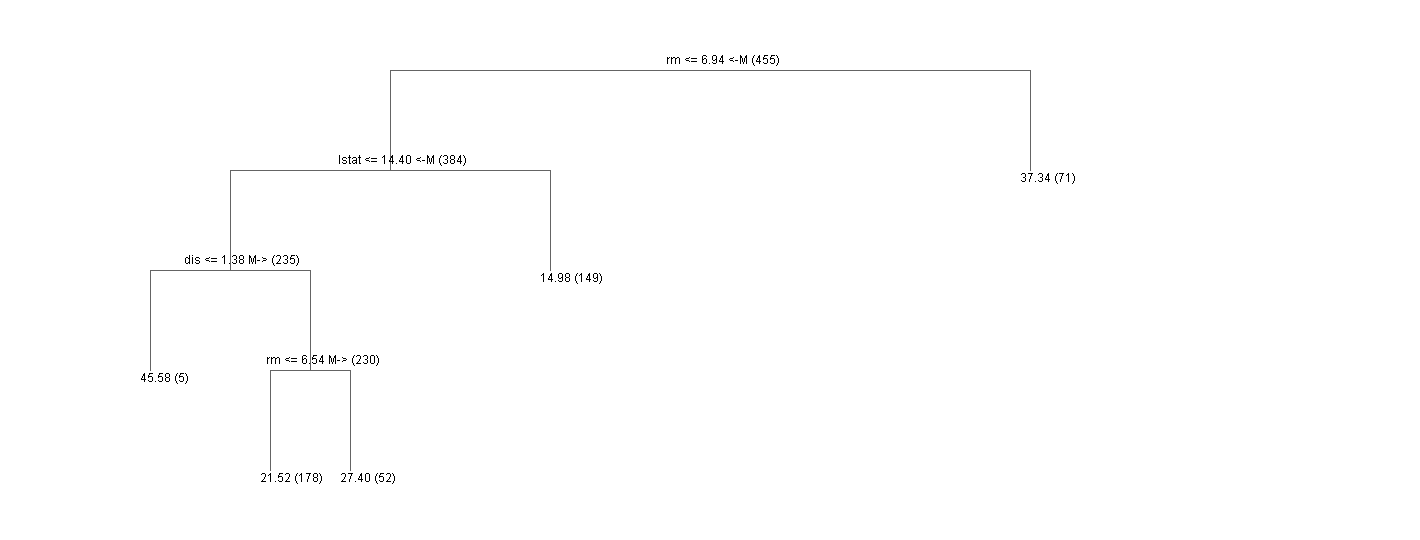
\includegraphics[width=9in]{yarf_mod_tree_1.png}
\end{figure}
\vspace{-1.2cm}
\benum

\subquestionwithpoints{12} Record the letter(s) of all the following that are \textbf{true}. 


\begin{enumerate}[(a)]
\item This tree model can be written as a linear model.
\item This tree model has 5 nodes.
\item This tree model has 5 root nodes.
\item This tree model splits $\mathcal{X}$ into rectangular prisms (i.e. dimension 3).
\item This tree model is overfit.
\item If you label the leaves 1,2 \ldots, L from left to right in the above, and you must split further on one of them, then splitting on leaf \#1 is most likely to yield a better tree model.
\item An OLS model will be more accurate out of sample than this model.
\item The most important feature in the data for predicting the response is \texttt{lstat}.
\item The model of the form $\yhat = b_0 + b_1 \u$ where is $\u$ restricted totr be one of the features in this dataset has highest $R^2$ when $\u$ is the variable \texttt{rm}.
\item The model of the form $\yhat = b_0 + b_1 \u$ where $\u$ is restricted to be dummy has highest $R^2$ when $\u$ is the computed via the function $\indic{rm \leq 6.94}$.
\item If \texttt{rm} = 7, the tree would predict 37.34 for $y$ regardless of the values of the other 12 features.
\item If \texttt{rm} = 6, the tree would predict $<$37.34 for $y$ regardless of the values of the other 12 features.
\end{enumerate}
\eenum\instr\pagebreak

%%%%%%%%%%%%%%%%%%%%%%%%

\problem [11min] Let $p=1$, $n > 100 + 1$, $d \in \braces{10, 11, \ldots, 100}$, $\mathcal{A}$ = OLS and consider the following different complexity sets that are used within the algorithm:

\beqn
\mathcal{H}_1 &=& \braces{w_0 + w_1 x_1 ~:~w_0, w_1 \in \reals}\\
\mathcal{H}_2 &=& \braces{w_0 + w_1 \natlog{x_1} ~:~w_0, w_1 \in \reals}\\
\mathcal{H}_3 &=& \braces{w_0 + w_1 x_1 + w_2 x^2 ~:~w_0, w_1, w_2 \in \reals}\\
\mathcal{H}_4 &=& \braces{w_0 + w_1 x_1 + w_2 x^2 + \ldots + w_d x^d ~:~w_0, w_1, \ldots, w_d \in \reals}\\
\eeqn

\vspace{-1cm}
\benum

\subquestionwithpoints{17} Record the letter(s) of all the following that are \textbf{true}. 


\begin{enumerate}[(a)]
\item The lowest RMSE will be from $\mathcal{H}_4$.
\item The lowest oos RMSE will be from $\mathcal{H}_4$.
\item The degrees of freedom in $\mathcal{H}_4$ equals $d$.
\item $b_1$ is the same in both $\mathcal{H}_1$ and $\mathcal{H}_3$.
\item If the response was logged, $b_1$ would be the same in both $\mathcal{H}_1$ and $\mathcal{H}_2$.
\item The design matrix for $\mathcal{H}_2$ looks like $\X = \bracks{\onevec_n, \bracks{\natlog{x_1}~\natlog{x_2} ~ \ldots ~ \natlog{x_n}}^\top}$.
\item The design matrix for $\mathcal{H}_3$ looks like $\X = \bracks{\onevec_n, \bracks{x_1^2~x_2^2 ~ \ldots ~ x_n^2}^\top}$.
\item In $\mathcal{H}_4$, if $d = 100$, then $R^2 = 100\%$.
\item In $\mathcal{H}_4$, if $d$ was set to be large, predictions for $\x_* \in \mathcal{X}$ will likely be more accurate than $\x_* \notin \mathcal{X}$.
\item In $\mathcal{H}_4$, if $d$ was set to be large, predictions for $\x_* \notin \mathcal{X}$ will likely be worse than if $d$ were set to be small.
\item In $\mathcal{H}_4$, if $d$ was varied across its range specified in the problem, then you can trace out the in-sample vs. oos complexity curve and locate the optimal model as a function of the hyperparameter $d$.
\item Assuming you do the procedure in the previous question and locate the optimal model given by $d = d^\star$, the oos $s_e$ from that procedure for the optimal model would be biased upwards.
\item The oos $s_e$ from that procedure for the optimal model would be biased downwards.\\

When comparing two mutually observed observations (A) and (B) sampled in the same fashion as those in $\mathbb{D}$, when the x measurement of (A) is \line(1,0){40}~ than the $x$ measurement of (B) then (A) is predicted to have a \line(1,0){40}~ from the (B)'s assuming the model is true. The blanks would be filled in by...

\item In $\mathcal{H}_1$, \qu{one unit larger} / \qu{response $y$ that differs by $b_1$}.

\item In $\mathcal{H}_2$, \qu{one unit larger} / \qu{response $y$ that differs by $b_1$}.
\item In $\mathcal{H}_2$, \qu{10\% larger} / \qu{response $y$ that differs by $0.1 b_1$}.
\item In $\mathcal{H}_2$, \qu{10\% larger} / \qu{response $y$ 10\% larger}.
\end{enumerate}
\eenum\instr\pagebreak

%%%%%%%%%%%%%%%%%%%%%%%%



\problem This question is about the concept of model validation and the strategy we discussed in class. Let's say we divide scramble the rows of $\mathbb{D}$ then create a partition 

\beqn
\mathbb{D} = \fivevec{\mathbb{D}_{\text{train}}}{\text{------}}{\mathbb{D}_{\text{select}}}{\text{------}}{\mathbb{D}_{\text{test}}}
\eeqn

\noindent in a 8:1:1 ratio train : select : test (in number of rows). We wish to select the best model $g_{m_*}$ out of $M$ candidate models $g_1, g_2, \ldots, g_M$ using the model selection procedure from class.

\benum
\subquestionwithpoints{12} Record the letter(s) of all the following that are \textbf{true}. 


\begin{enumerate}[(a)]
\item The three sets above could be permuted and the model selection procedure would still be valid.
\item The three sets above could be permuted and the model selection procedure would yield the same $g_{m_*}$.
\item The test set has 10\% of the total dataset.
\item The select set has 11.11\% of the total dataset.
\item When selecting models, the training data has 80\% of the data used for exclusively the selection step of the model selection procedure.
\item If we were to use only inner CV, then there would be a total of $K = 10$ folds.
\item If we were to use only outer CV, then there would be a total of $K = 10$ folds.
\item If we were to not use any CV, then we would get an estimate of the future performance of one specific $g_{m_*}$.
\item If we were to use only inner CV, then we would get an estimate of the future performance of one specific $g_{m_*}$.
\item If we were to use only outer CV, then we would get an estimate of the future performance of one specific $g_{m_*}$.
\item If we were to use both inner and outer CV, then we would get an estimate of the future performance of one specific $g_{m_*}$.
\item If $\mathbb{D}_{\text{train}}$ was reduced in size, then we increase misspecification error among all $M$ models during the model selection procedure.
\end{enumerate}
\eenum\instr\pagebreak

\end{document}

%%%%%%%%%%%%%%%%%%%%%%%%
%%%%%%%%%%%%%%%%%%%%%%%%
%%%%%%%%%%%%%%%%%%%%%%%%
%%%%%%%%%%%%%%%%%%%%%%%%
%%%%%%%%%%%%%%%%%%%%%%%%
%%%%%%%%%%%%%%%%%%%%%%%%